\documentclass{report}
\usepackage[utf8]{inputenc}
\usepackage{tabularx}
\usepackage{listings}
\usepackage{graphicx}
\usepackage{amsmath}
\usepackage{bm}
\usepackage{array}
\usepackage{amssymb}

\title{MAD 2019/2020 Exam Answers}
\author{Exam Number: 18}
\date{January 13, 2020}

\begin{document}

\maketitle

\subsection*{Exercise 1}
I find the task of this exercise a little ambiguous, as I am not sure if I am supposed to (only) compute the mean point of the data, the two eigenvalues and the two eigenvectors or if I am also supposed to convert the dimensionality. To be on the safe side, I will also convert the dimensionality, however, if I was not supposed to do this, please just overlook that part of my answer. \\
\\
We are given the following $N = 8$ 2-dimensional points:
\begin{center}
    \begin{tabular}{|l|l|l|l|l|l|l|l|l|}
        \hline
        coordinate x & 0.1 & 0.5 & 1.1 & -0.5 & 1.3 & 0.2 & -0.1 & 1 \\
        \hline
        coordinate y & 1 & 1 & 2 & 0.2 & -0.1 & -0.1 & -1.5 & -2.5 \\
        \hline
    \end{tabular}
\end{center}
First of we need to make each row have zero mean. This is done, by first computing $\bar{x}$ and $\bar{y}$:
$$\bar{x} = \frac{1}{8} \sum^8 _{n = 1} x_n = 0.45, \quad \quad \bar{y} = \frac{1}{8} \sum^8 _{n = 1} y_n = 0$$

\noindent Which gives us the mean point of data, $(0.45, 0)$. $\bar{x}$ and $\bar{y}$ are then subtracted from respectively coordinate x and coordinate y, which results in the following rows, with zero mean:
\begin{center}
    \begin{tabular}{|l|l|l|l|l|l|l|l|l|}
        \hline
        coordinate x & -0.35 & 0.05 & 0.65 & -0.95 & 0.85 & -0.25 & -0.55 & 0.55 \\
        \hline
        coordinate y & 1 & 1 & 2 & 0.2 & -0.1 & -0.1 & -1.5 & -2.5 \\
        \hline
    \end{tabular}
\end{center}
From this we can extract the following matrix:
\begin{center}
    \begin{math}
        \bm{S} = 
        \begin{bmatrix}
            -0.35 & 1 \\
            0.05 & 1 \\
            0.65 & 2 \\
            -0.95 & 0.2 \\
            0.85 & -0.1 \\
            -0.25 & -0.1 \\
            -0.55 & -1.5 \\
            0.55 & -2.5
        \end{bmatrix}
    \end{math}
\end{center}
Which we use to compute the covariance matric $\bm{C}$:
\begin{center}
    \begin{math}
        \bm{C} = \frac{1}{N} \cdot \bm{S}^T \cdot \bm{S}
        = \frac{1}{8} \cdot 
        \begin{bmatrix}
            -0.35 & 0.05 & 0.65 & -0.95 & 0.85 & -0.25 & -0.55 & 0.55 \\
            1 & 1 & 2 & 0.2 & -0.1 & -0.1 & -1.5 & -2.5
        \end{bmatrix}
        \cdot 
        \begin{bmatrix}
            -0.35 & 1 \\
            0.05 & 1 \\
            0.65 & 2 \\
            -0.95 & 0.2 \\
            0.85 & -0.1 \\
            -0.25 & -0.1 \\
            -0.55 & -1.5 \\
            0.55 & -2.5
        \end{bmatrix} \newline
        =
        \begin{bmatrix}
            0.355 & 0.025 \\
            0.025 & 1.82
        \end{bmatrix}
    \end{math}
\end{center}
Now that we have found the covariance matrix $\bm{C}$, we can find the eigenvalues. First we need to compute $\bm{C}-\lambda \cdot \bm{I}_2$:
\begin{center}
    \begin{math}
        \bm{C} - \lambda \cdot \bm{I}_2 =
        \begin{bmatrix}
            0.355 & 0.025 \\
            0.025 & 1.82
        \end{bmatrix}
        -
        \begin{bmatrix}
            \lambda & 0 \\
            0 & \lambda
        \end{bmatrix}
        =
        \begin{bmatrix}
            0.355 - \lambda & 0.025 \\
            0.025 & 1.82 - \lambda
        \end{bmatrix}
    \end{math}
\end{center}
Which we need to find the determinant of:
\begin{center}
    \begin{math}
        det(\bm{C}-\lambda \cdot \bm{I}_2) = 
        \begin{vmatrix}
            0.355 - \lambda & 0.025 \\
            0.025 & 1.82 - \lambda
        \end{vmatrix} \newline
        =
        (0.355 - \lambda) \cdot (1.82 - \lambda) - 0.025 * 0.025 \newline
        = 0.355 \cdot 1.82 - \lambda \cdot 1.82 + \lambda^2 - 0.025 \cdot 0.025 - 0.355 \cdot \lambda \newline
        \approx \lambda^2 - 2.175 \lambda + 0.6455
    \end{math}
\end{center}
And now solve for $\lambda$:
$$\lambda^2 - 2.175 \lambda + 0.6455 = 0$$
$\Leftrightarrow$
$$\lambda \ \frac{-(-2.175) \pm \sqrt{(-2.175)^2 - 4 \cdot 1 \cdot 0.6455}}{2 \cdot 1} \approx 
\begin{cases}
    1.820 \\
    0.355
\end{cases}$$
Thus, we have found the two eigenvalues $\lambda_1 = 1.820$ and $\lambda_2 = 0.355$. \\

Now, for finding the associated eigenvectors, we first let $\lambda = \lambda_1$ and find $\bm{B} = \bm{C} - \lambda \cdot \bm{I}_2$:
\begin{center}
    \begin{math}
        \bm{B} = \bm{C} - \lambda \cdot \bm{I}_2 =
        \begin{bmatrix}
            0.355 - 1.820 & 0.025 \\
            0.025 & 1.82 - 1.820
        \end{bmatrix}
        \newline =
        \begin{bmatrix}
            -1.4658 & 0.025 \\
            0.025 & 0 \\
        \end{bmatrix}
    \end{math}
\end{center}
Now, we put $\bm{B} \bm{x} = \bm{0}$ on row echelon form
$$\bm{B} \bm{x} = \bm{0}$$
$\Rightarrow$
\begin{center}
    \begin{math}
        \left[
            \begin{array}{cc|c}
                -1.4658 & 0.025 & 0 \\
                0.025 & 0 & 0 \\
            \end{array}
        \right]
    \end{math}
\end{center}
Which is done by adding row 1 times 0.0171 to row 2. Thus, we get the following augmented matrix:
\begin{center}
    \begin{math}
        \left[
            \begin{array}{cc|c}
                -1.4658 & 0.025 & 0 \\
                0 & 0 & 0 \\
            \end{array}
        \right]
    \end{math}
\end{center}
Thus, we have the following equation, where we isolate $x_1$:
$$-1.4658 \cdot x_1 + 0.025 \cdot x_2 = 0$$
$\Leftrightarrow$
$$0.025 \cdot x_2 = 1.4658 \cdot x_1$$
$\Leftrightarrow$
$$0.171 \cdot x_2 = x_1$$
From this point, we can choosing any integer for $x_2$ and get the eigenvector for the eigenvalue $1.820$. I am here choosing $x_2 = 1$:
$$0.171 \cdot 1 = x_1$$
$\Leftrightarrow$
$$0.171 = x_1$$
Thus, the eigenvector for the eigenvalue $1.820$ is:
\begin{center}
    \begin{math}
        \left[
            \begin{array}{c}
                0.171 \\
                1
            \end{array}
        \right]
    \end{math}
\end{center}

Now, we let $\lambda = \lambda_2$ and follow the same procedure:
\begin{center}
    \begin{math}
        \bm{B} = \bm{C} - \lambda \cdot \bm{I}_2 =
        \begin{bmatrix}
            0.355 - 0.355 & 0.025 \\
            0.025 & 1.82 - 0.355
        \end{bmatrix}
        \newline =
        \begin{bmatrix}
            0 & 0.025 \\
            0.025 & 1.465 \\
        \end{bmatrix}
    \end{math}
\end{center}
$$\bm{B} \bm{x} = \bm{0}$$
$\Rightarrow$
\begin{center}
    \begin{math}
        \left[
        \begin{array}{cc|c}
            0 & 0.025 & 0 \\
            0.025 & 1.465 & 0 \\
        \end{array}
        \right]
    \end{math}
\end{center}
To put the matrix on row echelon form, we simply swap row 1 and row 2 and optain the following matrix
\begin{center}
    \begin{math}
        \left[
        \begin{array}{cc|c}
            0.025 & 1.465 & 0 \\
            0 & 0.025 & 0 \\
        \end{array}
        \right]
    \end{math}
\end{center}
Thus, we have the following equation, where $x_1$ needs to be isolated:
$$0.025 \cdot x_1 + 1.465 \cdot x_2 = 0$$
$\Leftrightarrow$
$$1.465 \cdot x_2 = -0.025 \cdot x_1$$
$\Leftrightarrow$
$$ -58.6 \cdot x_2 = x_1$$
Again, here it is possible to choose any value for $x_2$, I will let $x_2 = 1$ and get the following:
$$ -58.6 \cdot 1 = x_1$$
$\Leftrightarrow$
$$ -58.6 = x_1$$
Thus, for the eigenvalue 0.355, we have the eigenvector
\begin{center}
    \begin{math}
        \left[
            \begin{array}{c}
                -58.6 \\
                1
            \end{array}
        \right]
    \end{math}
\end{center}
Thus, sorting the eigenvalues in descending order and the eigenvectors accordingly, we get the following matrix of the eigenvectors:
\begin{center}
    \begin{math}
        \bm{P} =
        \left[
            \begin{array}{cc}
                0.171 & -58.6 \\
                1 & 1
            \end{array}
        \right]
    \end{math}
\end{center}
The dimensionality of the given data can now be converted by multiplying the zero-mean matrix, $\bm{S}$ with $\bm{P}$:
\begin{center}
    \begin{math}
        \begin{bmatrix}
            -0.35 & 1 \\
            0.05 & 1 \\
            0.65 & 2 \\
            -0.95 & 0.2 \\
            0.85 & -0.1 \\
            -0.25 & -0.1 \\
            -0.55 & -1.5 \\
            0.55 & -2.5
        \end{bmatrix}
        \cdot
        \left[
            \begin{array}{cc}
                0.171 & -58.6 \\
                1 & 1
            \end{array}
        \right]
        =
        \begin{bmatrix}
            0.9402 & 21.51 \\
            1.0086 & -1.93 \\
            2.1112 & -36.09 \\
            0.03755 & 55.87 \\
            0.04535 & -49.91 \\
            -0.1428 & 14.55 \\
            -1.5941 & 30.73 \\
            -2.406 & -34.73
        \end{bmatrix}
    \end{math}
\end{center}

\section*{Exercise 2}
First, we compute $Gini(T_{org}, \lambda)$:
$$Gini(T_{org}, \lambda) = \frac{17}{28} \cdot gini(T_{first}) + \frac{11}{28} \cdot gini(T_{second})$$
$$= \frac{17}{28} \left(1 - \left(\frac{6}{17}\right)^2 - \left( \frac{1}{17} \right)^2 - \left( \frac{10}{17} \right)^2 \right) + \frac{11}{28} \left(1 - \left( \frac{1}{11} \right)^2 - \left( \frac{7}{11} \right)^2 - \left( \frac{3}{11} \right)^2 \right)$$
$$ = 0.5206$$

Next, we compute $Gain(T_{orig}, \lambda)$:
$$Gain(T_{orig}, \lambda) = H(7, 8, 13) - \frac{17}{28} \cdot H(6, 1, 10) - \frac{11}{28} \cdot H(1, 7, 3)$$
$$ = \left(-\frac{13}{28} \cdot \log_2 \left(\frac{13}{28} \right) - \frac{8}{28} \cdot \log_2 \left( \frac{8}{28} \right) - \frac{7}{28} \cdot \log_2 \left( \frac{7}{28} \right) \right)$$
$$ - \frac{17}{28} \left( - \frac{10}{17} \cdot \log_2 \left( \frac{10}{17} \right) - \frac{6}{17} \cdot \log_2 \left( \frac{6}{17} \right) - \frac{1}{17} \cdot \log_2 \left( \frac{1}{17} \right) \right)$$
$$ - \frac{11}{28} \left( - \frac{7}{11} \cdot \log_2 \left( \frac{7}{11} \right) - \frac{3}{11} \cdot \log_2 \left( \frac{3}{11} \right) - \frac{1}{11} \cdot \log_2 \left( \frac{1}{11} \right) \right)$$
$$= 0.3015$$

Thus, it has been computed, that $Gini(T_{org}, \lambda) = 0.5206$ and $Gain(T_{orig}, \lambda) = 0.3015$

\subsection*{Exercise 3}
With my implementation, I have the following performance of the cross-validation:
\begin{center}
    \begin{tabular}{|l|l|}
        \hline
        C & Accuracy \\
        \hline
        0.001 & 0.9225 \\
        \hline
        0.01 & 0.92125 \\
        \hline
        0.1 & 0.9274999999999999 \\
        \hline
        1 & 0.9237500000000001 \\
        \hline
        10 & 0.9237500000000001 \\
        \hline
        100 & 0.9237500000000001 \\
        \hline
    \end{tabular}
\end{center}
And the following decision boundary for the optimal svm classifier:
\begin{center}
    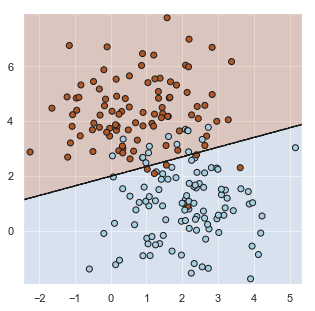
\includegraphics[height = 7 cm]{3_decision_boundary.png}
\end{center}

\section*{Exercise 4}
\subsection*{Part 1}
\subsubsection*{(a)}
With my implementation, I have gotten the following RMSE-value:
$$RMSE = 0.8243064553494787$$
And the following scatter plot:
\begin{center}
    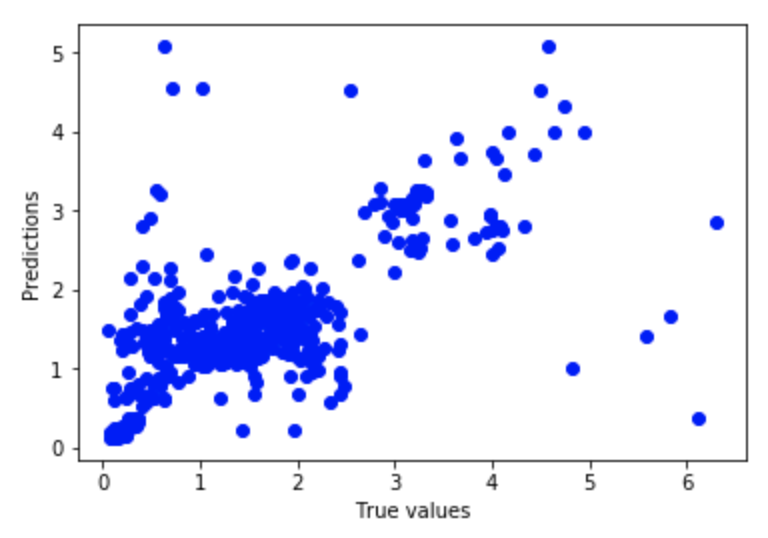
\includegraphics[height = 7 cm]{kNN_Scatter_a}
\end{center}

\subsubsection*{(b)}
With this new distance formula, I have optained the following RMSE-value:
$$RMSE = 1.0997971796682453$$
And the following scatter plot:
\begin{center}
    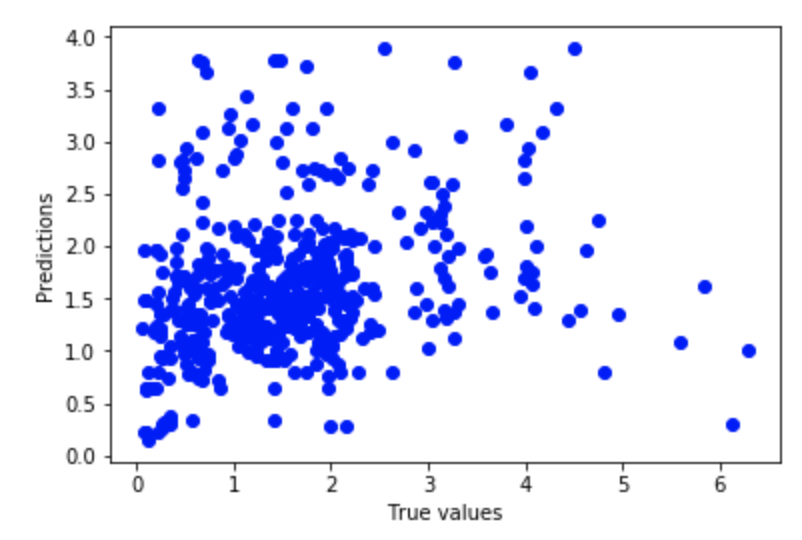
\includegraphics[height = 7 cm]{kNN_Scatter_b}
\end{center}
The matrix \textit{M}, makes it possible to tune the impact that the different features have on the distance between the two data point, thus also the impact on the prediction. For instance, the given example matrix
\begin{center}
    \begin{math}
        \left[
        \begin{array}{cccccccccc}
            0.00001 & 0 & 0 & 0 & 0 & 0 & 0 & 0 & 0 & 0 \\
            0 & 0.00001 & 0 & 0 & 0 & 0 & 0 & 0 & 0 & 0 \\
            0 & 0 & 0.00001 & 0 & 0 & 0 & 0 & 0 & 0 & 0 \\
            0 & 0 & 0 & 0.00001 & 0 & 0 & 0 & 0 & 0 & 0 \\
            0 & 0 & 0 & 0 & 0.00001 & 0 & 0 & 0 & 0 & 0 \\
            0 & 0 & 0 & 0 & 0 & 0.00001 & 0 & 0 & 0 & 0 \\
            0 & 0 & 0 & 0 & 0 & 0 & 0.00001 & 0 & 0 & 0 \\
            0 & 0 & 0 & 0 & 0 & 0 & 0 & 0.00001 & 0 & 0 \\
            0 & 0 & 0 & 0 & 0 & 0 & 0 & 0 & 1.0 & 0 \\
            0 & 0 & 0 & 0 & 0 & 0 & 0 & 0 & 0 & 1.0 \\
        \end{array}
        \right]
    \end{math}
\end{center}
makes the two last features have a bigger impact on the distance and prediction, than the first eight features. This could imply, that the two last feature are more "important", than the first eight features.
\subsection*{Part 2}
With my implementation, I got the following RMSE-value:
$$RMSE = 0.8925765347348245$$
And the following scatter plot:
\begin{center}
    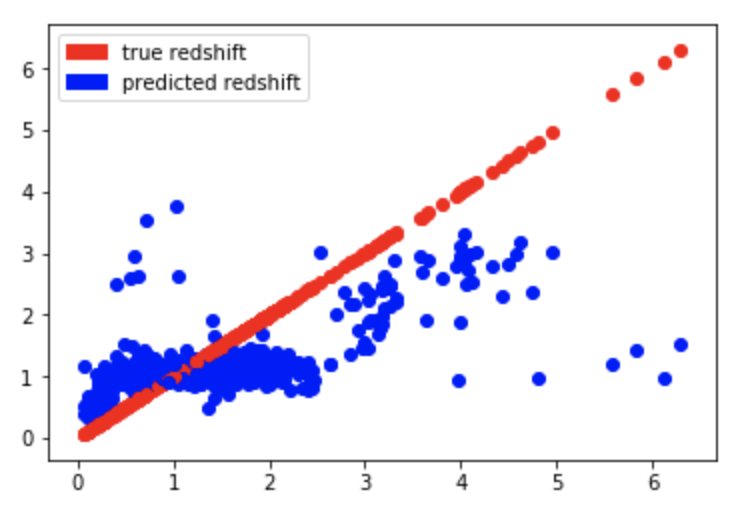
\includegraphics[height = 7 cm]{LinRegNeighbors_scatter.png}
\end{center}

\section*{Exercise 5}
\subsection*{Part 1}
We have been given the following expression
\begin{center}
    \begin{math}
        p(t_n|\bm{x}_n; \bm{w}) = \frac{f(\bm{x}_n; \bm{w})^{t_n}exp(-f(\bm{x}_n; \bm{w}))}{t_n!}
    \end{math}
\end{center}
And we wish to find the joint conditional density:
\begin{center}
    \begin{math}
        p(\bm{t}|\bm{X};\bm{w})
    \end{math}
\end{center}
Which extends to
\begin{center}
    \begin{math}
        p(t_1, ..., t_N | \bm{x}_1, ..., \bm{x}_N; \bm{w})
    \end{math}
\end{center}
Following the formula for joint probability distribution
\begin{center}
    \begin{math}
        p(A, B) = p(A) \cdot p(B)
    \end{math}
\end{center}
We get the result
\begin{center}
    \begin{math}
        p(\bm{t}|\bm{X};\bm{w}) = \displaystyle\prod_{n = 1}^N p(t_n|\bm{x}_n; \bm{w}) = \displaystyle\prod_{n = 1}^N \frac{f(\bm{x}_n; \bm{w})^{t_n}exp(-f(\bm{x}_n; \bm{w}))}{t_n!}
    \end{math}
\end{center}

\subsection*{Part 2}
Since, it says in the exercise desciption, how we only should include the essential steps for deriving the expression, some of the descriptions of actions in the following exercise have been left out. \\
We have been given the expression for $p(w | \bm{t}, \bm{X}, \mu_0, \sigma_0^2)$, which we extend
\begin{center}
    \begin{math}
        p(w | \bm{t}, \bm{X}, \mu_0, \sigma_0^2) = \frac{\prod_{n = 1}^N \left( \frac{f(\bm{x}_n; \bm{w})^{t_n}exp(-f(\bm{x}_n; \bm{w}))}{t_n!}\right) \frac{1}{(2 \pi)^\frac{D+1}{2} \det(\sigma_0^2 \bm{I})^\frac{1}{2}} \exp(-\frac{1}{2}(\bm{w} - \mu_0)^T(\sigma_0^2\bm{I})^{-1}(\bm{w} - \mu_0))}{p(\bm{t} | \bm{X})}
    \end{math}
\end{center}
To find $\log p(w | \bm{t}, \bm{X}, \mu_0, \sigma_0^2)$, we start of by taking the $\log$ on both sides and reducing a little:
\begin{center}
    \begin{math}
        \log p(w | \bm{t}, \bm{X}, \mu_0, \sigma_0^2) = 
        \log \left(\frac{\prod_{n = 1}^N \left( \frac{f(\bm{x}_n; \bm{w})^{t_n}\exp(-f(\bm{x}_n; \bm{w}))}{t_n!}\right) \frac{1}{(2 \pi)^\frac{D+1}{2} \det(\sigma_0^2 \bm{I})^\frac{1}{2}} \exp(-\frac{1}{2}(\bm{w} - \mu_0)^T(\sigma_0^2\bm{I})^{-1}(\bm{w} - \mu_0))}{p(\bm{t} | \bm{X})} \right) \newline
        = \log \left( \prod_{n = 1}^N \left( \frac{f(\bm{x}_n; \bm{w})^{t_n}\exp(-f(\bm{x}_n; \bm{w}))}{t_n!}\right) \right) + 
        \log \left( \frac{1}{(2 \pi)^\frac{D+1}{2} \det(\sigma_0^2 \bm{I})^\frac{1}{2}} \right) 
        + \log \left( \exp(-\frac{1}{2}(\bm{w} - \mu_0)^T(\sigma_0^2\bm{I})^{-1}(\bm{w} - \mu_0)) \right) 
        - \log \left( p(\bm{t} | \bm{X}) \right)
    \end{math}
\end{center}
For the sake of readability, I choose to split the proof into three sections:
\subsubsection*{First Section}
In this section, I will prove 
\begin{center}
    \begin{math}
        \log \left( \prod_{n = 1}^N \left( \frac{f(\bm{x}_n; \bm{w})^{t_n}\exp(-f(\bm{x}_n; \bm{w}))}{t_n!}\right) \right) = \sum^N_{n = 1} \left( t_n \log f(\bm{x}_n; \bm{w}) - f(\bm{x}_n; \bm{w}) - \log t_n ! \right)
    \end{math}
\end{center}
This is done by the following
\begin{center}
    \begin{math}
        \log \left( \prod_{n = 1}^N \left( \frac{f(\bm{x}_n; \bm{w})^{t_n}\exp(-f(\bm{x}_n; \bm{w}))}{t_n!}\right) \right)
        = \sum^N_{n = 1} \log \left( \frac{f(\bm{x}_n; \bm{w})^{t_n}\exp(-f(\bm{x}_n; \bm{w}))}{t_n!}\right) 
        = \sum^N_{n = 1} \left( \log(f(\bm{x}_n; \bm{w})^{t_n}\exp(-f(\bm{x}_n; \bm{w}))) - \log t_n! \right)
        = \sum^N_{n = 1} \left( \log f(\bm{x}_n; \bm{w})^{t_n} + \log \exp(-f(\bm{x}_n; \bm{w})) - \log t_n! \right)
        = \sum^N_{n = 1} \left( t_n \log f(\bm{x}_n; \bm{w}) -f(\bm{x}_n; \bm{w}) - \log t_n! \right)
    \end{math}
\end{center}

\subsubsection*{Second Section}
In this section, I will prove 
\begin{center}
    \begin{math}
        \log \left( \exp(-\frac{1}{2}(\bm{w} - \mu_0)^T(\sigma_0^2\bm{I})^{-1}(\bm{w} - \mu_0)) \right) 
        = -\frac{1}{2 \sigma_0^2}(\bm{w} - \mu_0)^T (\bm{w} - \mu_0)
    \end{math}
\end{center}
This is done by
\begin{center}
    \begin{math}
        \log \left( \exp(-\frac{1}{2}(\bm{w} - \mu_0)^T(\sigma_0^2\bm{I})^{-1}(\bm{w} - \mu_0)) \right) 
        = -\frac{1}{2}(\bm{w} - \mu_0)^T(\sigma_0^2\bm{I})^{-1}(\bm{w} - \mu_0)
        = -\frac{1}{2}(\bm{w} - \mu_0)^T(\frac{1}{\sigma_0^2}\bm{I})(\bm{w} - \mu_0)
        = -\frac{1}{2} \frac{1}{\sigma_0^2} (\bm{w} - \mu_0)^T\bm{I}(\bm{w} - \mu_0)
        = -\frac{1}{2 \sigma_0^2} (\bm{w} - \mu_0)^T(\bm{w} - \mu_0)
    \end{math}
\end{center}

\subsubsection*{Third section}
In this section, I will prove
\begin{center}
    \begin{math}
        \log \left( \frac{1}{(2 \pi)^\frac{D+1}{2} \det(\sigma_0^2 \bm{I})^\frac{1}{2}} \right) 
        = - \log \left( \sqrt{2 \pi \sigma_0^2}^{D + 1} \right)
    \end{math}
\end{center}
This is done by
\begin{center}
    \begin{math}
        \log \left( \frac{1}{(2 \pi)^\frac{D+1}{2} \det(\sigma_0^2 \bm{I})^\frac{1}{2}} \right) 
        = \log(1) - \log((2 \pi)^\frac{D+1}{2} \det(\sigma_0^2 \bm{I})^\frac{1}{2})
        = - \log((2 \pi)^\frac{D+1}{2} \left( \sigma_0^{2 \cdot (D + 1)} \right)^\frac{1}{2})
        = - \log((2 \pi)^\frac{D+1}{2} \left( \sigma_0^{2} \right)^\frac{D + 1}{2})
        = - \log((2 \pi)^{\left(\frac{1}{2}\right)^D} \left( \sigma_0^{2} \right)^{\left(\frac{1}{2}\right)^D})
        = - \log (2 \pi \sigma_0^{2})^{\left(\frac{1}{2}\right)^D}
        = - \log \sqrt{(2 \pi \sigma_0^{2})}^D
    \end{math}
\end{center}

\subsubsection{}

Substituting the results of these three sections into $\log p(w | \bm{t}, \bm{X}, \mu_0, \sigma_0^2)$ gives the following
\begin{center}
    \begin{math}
        \log p(w | \bm{t}, \bm{X}, \mu_0, \sigma_0^2)
        = \log \left( \prod_{n = 1}^N \left( \frac{f(\bm{x}_n; \bm{w})^{t_n}\exp(-f(\bm{x}_n; \bm{w}))}{t_n!}\right) \right) + 
        \log \left( \frac{1}{(2 \pi)^\frac{D+1}{2} \det(\sigma_0^2 \bm{I})^\frac{1}{2}} \right) 
        + \log \left( \exp(-\frac{1}{2}(\bm{w} - \mu_0)^T(\sigma_0^2\bm{I})^{-1}(\bm{w} - \mu_0)) \right) 
        - \log \left( p(\bm{t} | \bm{X}) \right)
        = \sum^N_{n = 1} \left( t_n \log f(\bm{x}_n; \bm{w}) -f(\bm{x}_n; \bm{w}) - \log t_n! \right) - \log \sqrt{(2 \pi \sigma_0^{2})}^D -\frac{1}{2 \sigma_0^2} (\bm{w} - \mu_0)^T(\bm{w} - \mu_0) - \log \left( p(\bm{t} | \bm{X}) \right)
    \end{math}
\end{center}
Rearranging, the equation a little, and we get to the result:
\begin{center}
    \begin{math}
        \displaystyle \sum^N_{n = 1} \left( t_n \log f(\bm{x}_n; \bm{w}) -f(\bm{x}_n; \bm{w}) - \log t_n! \right) - \log \sqrt{(2 \pi \sigma_0^{2})}^D -\frac{1}{2 \sigma_0^2} (\bm{w} - \mu_0)^T(\bm{w} - \mu_0) - \log \left( p(\bm{t} | \bm{X}) \right) \newline
        = \displaystyle \sum^N_{n = 1} \left( t_n \log f(\bm{x}_n; \bm{w}) -f(\bm{x}_n; \bm{w}) - \log t_n! \right) -\frac{1}{2 \sigma_0^2} (\bm{w} - \mu_0)^T(\bm{w} - \mu_0) - \log \sqrt{(2 \pi \sigma_0^{2})}^D - \log \left( p(\bm{t} | \bm{X}) \right),
        \quad \quad Q.E.D
    \end{math}
\end{center}
\end{document}